\documentclass{article}

% Packages
\usepackage{fancyhdr}
\usepackage{titlesec}
\usepackage{hyperref}
\usepackage{amsmath}
\usepackage{listings}
\usepackage{xcolor}
\usepackage{graphicx}
\usepackage{subfig}

%
% Basic Document Settings
%
\pagestyle{fancy}
\lstset{
	columns=fixed,       
	numbers=left,                                        
	numberstyle=\tiny\color{gray},                       
	frame=none,                                          
	backgroundcolor=\color[RGB]{245,245,244},           
	keywordstyle=\color[RGB]{40,40,255},                 
	numberstyle=\footnotesize\color{darkgray},           
	commentstyle=\it\color[RGB]{0,96,96},                
	stringstyle=\rmfamily\slshape\color[RGB]{128,0,0},   
	showstringspaces=false,                              
	language=R,   
	breaklines,                                     
}

%
% Assignment Details
%   - Title
%   - Class
%   - Instructor
%   - Due date
%   - Author
%
\newcommand{\asgmTitle}{Assignment}
\newcommand{\asgmClass}{Operational Statistics for SAR Imagery}
\newcommand{\asgmInstructor}{Professor Alejandro C.\ Frery}
\newcommand{\asgmDueDate}{July 28, 2019}
\newcommand{\asgmAuther}{Zhangyue Xiong}
\newcommand{\StudentID}{23020181154246}

%
% Title Page
%
\title{
	\vspace{2in}
	\textmd{\textbf{\asgmTitle}}\\
	\vspace{0.1in}\large{\textbf{\asgmClass}}\\
	\vspace{0.1in}\large{\textit{\asgmInstructor}}\\
	\vspace{3in}
}
\author{\vspace{0.1in}\textbf{\asgmAuther}\\ \textbf{\StudentID}}
\date{\today}

\begin{document}

\maketitle
\thispagestyle{empty}

\pagebreak
\setcounter{page}{0}
\thispagestyle{empty}
\tableofcontents


% Create Assignment Sections

% Assignment 1 
\pagebreak
\setcounter{page}{1}
\section*{Assignment \#1}
\addcontentsline{toc}{section}{Assignment \#1}
\subsection*{Task}
\addcontentsline{toc}{subsection}{Task}
Read, summarize and comment this article \cite{almeida2012good}.
\subsection*{Summary and Comment}
\addcontentsline{toc}{subsection}{Summary and Comment}
%1. Why did the authors bother to write this paper?
Mathematical modelling aims at solving complex problems which can be described in a rigorous mathematical way that enables the use of computers for finding the solution. 
There are high number of variables requires strong computational effort in their solutions. 
In complex problems, there are many variables and values. minute errors in obtaining the eigenvalue and eigenvector or a matrix determinant, in calculating an average, a standard deviation or correlation coefficient, can lead to erroneous.
To search for best approximate solutions, we need to consider some reasonable bounds of errors, imposes tight accuracy requirements on the computational platforms and its libraries or functions.  
However, little attention has been drawn to assess different platforms under the diversity of operational systems and hardware considering the accuracy of the results. 
Authers aim to test the accuracy of different platforms used in computational modeling, running on the same operational system and hardware.\\
%2. How did they try to answer the question?
\\
They test the accuracy of three platforms used in computational modelling: MatLab, Octave and Scilab, running on i386 architecture and three operating systems(Windows, Ubuntu and Mac OS). They submitted them to numerical tests using standard data sets and using the function provided by each platform. In order to verify the stability of the results with respect to small departures from the original input, a Monte Carlo study was conducted in some of the datasets. They also used data provided by NIST(National Institute of Standards and Technology), a protocol which includes the computation of basic univariate statistics, linear regression and extremes of probability distributions.\\
%3. Which are the main results?
\\
The assessment was made comparing the results computed by the platforms with certified values, that is, known results, computing the number of correct significant digits. Regarding the computation of basic statics, Scilab is not only the worst performance platform but also the worst platform with respect to the stability of the results. Scilab presented the best performance when dealing with the binomial and t-Student deviation, and also when computing the cumulative distribution function of the Possion Law. When computing the F distributions, Octave produced the best result. Regrading the normal distribution, MatLab and Octave obtained the same good results, while Scilab produced bad results. The three platforms were acceptable when dealing with the gamma law. Matlab and Octave failed at computing the t-Student distribution. No single platform can be advised as safe for the linear regression problems here considered. Regarding the variability among operating systems, MatLab and Octave were equivalent and more consistent than Scilab in most of the situations under assessment.\\
%4. Is this relevant for me, or will it be in the future?
\\
I think the results of this article will provide some suggestions for selecting computational platforms in my future research.

% Assignment 2 
\section*{Assignment \#2}
\addcontentsline{toc}{section}{Assignment \#2}
\subsection*{Task}
\addcontentsline{toc}{subsection}{Task}
\paragraph{Exercise 4.4.} Obtain the expression of the density of $\mathcal K$-distributed
amplitude data via the transformation $Z_{A} = \sqrt{Z_{I}}$. Compute its moments.
Illustrate.
\paragraph{Exercise 4.8.} Obtain the expression of the density of $\mathcal G^{0}$-distributed amplitude data via the transformation $Z_{A} = \sqrt{Z_{I}}$. Compute its moments.
Illustrate.
\subsection*{Answer}
\addcontentsline{toc}{subsection}{Answer}
\textbf{Exercise 4.4. \\}
The density of $\mathcal K$-distributed:
\begin{displaymath}
f_{Z_I}(z_I;\alpha,\lambda,L) = \frac{2\lambda L}{\Gamma(\alpha)\Gamma(L)} (\lambda L z_I)^{\frac{\alpha+L}{2}-1} K_{\alpha-L}(2\sqrt{\lambda L z_I})
\end{displaymath}
When $Z_{A} = \sqrt{Z_{I}}$, which is $z_{I} = z_{A}^2$, the density of amplitude data $Z_A$ is:
\begin{displaymath}
\begin{split}
f_{Z_A}(z_A;\alpha,\lambda,L) =& \frac{2 \lambda L}{\Gamma(\alpha) \Gamma(L)}(z_A^2)'(\lambda L z_A^2)^{\frac{\alpha+L}{2}-1} K_{\alpha-L}{2\sqrt{\lambda L z_A^2}} \\
=& \frac{2 \lambda L}{\Gamma(\alpha) \Gamma(L)}2z_A(\lambda L z_A^2)^{\frac{\alpha+L}{2}-1}K_{\alpha-L}{2\sqrt{\lambda L z_A^2}} \\
=& \frac{4 \lambda L}{\Gamma(\alpha) \Gamma(L)}(\lambda L)^{\frac{\alpha+L}{2}-1}z_A^{\alpha+L-1}K_{\alpha-L}{2\sqrt{\lambda L z_A^2}}
\end{split}
\end{displaymath}
The $k$-order moments of $Z_I$ are:
\begin{displaymath}
E(Z_I^k) = (\lambda L)^{-k}{\frac{\Gamma(L+k)\Gamma(\alpha+k)}{\Gamma(L)\Gamma(\alpha)}}
\end{displaymath}
The $k$-order moments of $Z_A$ are:
\begin{displaymath}
\begin{split}
E(Z_A^k) =& E(Z_I^{\frac{k}{2}}) \\
=& (\lambda L)^{-\frac{k}{2}}{\frac{\Gamma(L+{\frac{k}{2}})\Gamma(\alpha+\frac{k}{2})}{\Gamma(L)\Gamma(\alpha)}}
\end{split}
\end{displaymath}
\textbf{Exercise 4.8. \\}
The the density of $\mathcal G^0$ distribution:
\begin{displaymath}
f_{Z_I}(z_I; \alpha,\gamma,L) = \frac{L^L \Gamma(L-\alpha)}{\gamma^\alpha \Gamma(L)\Gamma(-\alpha)} \frac{z_I^{L-1}}{(\gamma+L z_I)^{L-\alpha'}}
\end{displaymath}
When $Z_{A} = \sqrt{Z_{I}}$, which is $z_{I} = z_{A}^2$, the density of amplitude data $Z_A$ is:
\begin{displaymath}
\begin{split}
f_{Z_A}(z_A;\alpha,\gamma,L) =& \frac{L^L \Gamma(L-\alpha)}{\gamma^\alpha \Gamma(L)\Gamma(-\alpha)}{(z_A^2)'} \frac{(z_A^2)^{L-1}}{(\gamma+{L z_A^2})^{L-\alpha'}} \\
=& \frac{L^L \Gamma(L-\alpha)}{\gamma^\alpha \Gamma(L)\Gamma(-\alpha)}{2 z_A} \frac{(z_A^2)^{L-1}}{(\gamma+{L z_A^2})^{L-\alpha'}} \\
=& \frac{2 L^L \Gamma(L-\alpha)}{\gamma^\alpha \Gamma(L)\Gamma(-\alpha)} \frac{z_A^{2L-1}}{(\gamma+{L z_A^2})^{L-\alpha'}} \\
\end{split}
\end{displaymath}
The $k$-order moments of $Z_I$ are:
\begin{displaymath}
E(Z_I^k) = (\gamma / L)^{k} \frac{\Gamma(L+k)\Gamma(-\alpha-k)}{\Gamma(L)\Gamma(-\alpha)}
\end{displaymath}
The $k$-order moments of $Z_A$ are:
\begin{displaymath}
\begin{split}
E(Z_A^k) =& E(Z_I^{\frac{k}{2}}) \\
=& (\gamma / L)^{\frac{k}{2}} \frac{\Gamma(L+\frac{k}{2})\Gamma(-\alpha-\frac{k}{2})}{\Gamma(L)\Gamma(-\alpha)}
\end{split}
\end{displaymath}

% Assignment 3
\section*{Assignment \#3}
\addcontentsline{toc}{section}{Assignment \#3}
\subsection*{Task}
\addcontentsline{toc}{subsection}{Task}
Including today's activities
\subsection*{Activities}
\addcontentsline{toc}{subsection}{Activities}
\textbf{Test function} \\
Try to implement some function using R language 
\begin{lstlisting}
require(ggplot2)
require(ggthemes)

# square function

f.square <- function(x){
x^2
}
ggplot(data = data.frame(x = seq(-pi,pi,length.out = 500)),aes(x=x)) +
stat_function(fun = f.square, geom = "line", size=2, col="black") +
theme_classic() + 
theme(text = element_text(size = 20)) +
xlab("x") + ylab("Square")
ggsave(file = "F:/assignment/Figures/square.pdf")
\end{lstlisting}
\begin{figure}[hbt]
\centering
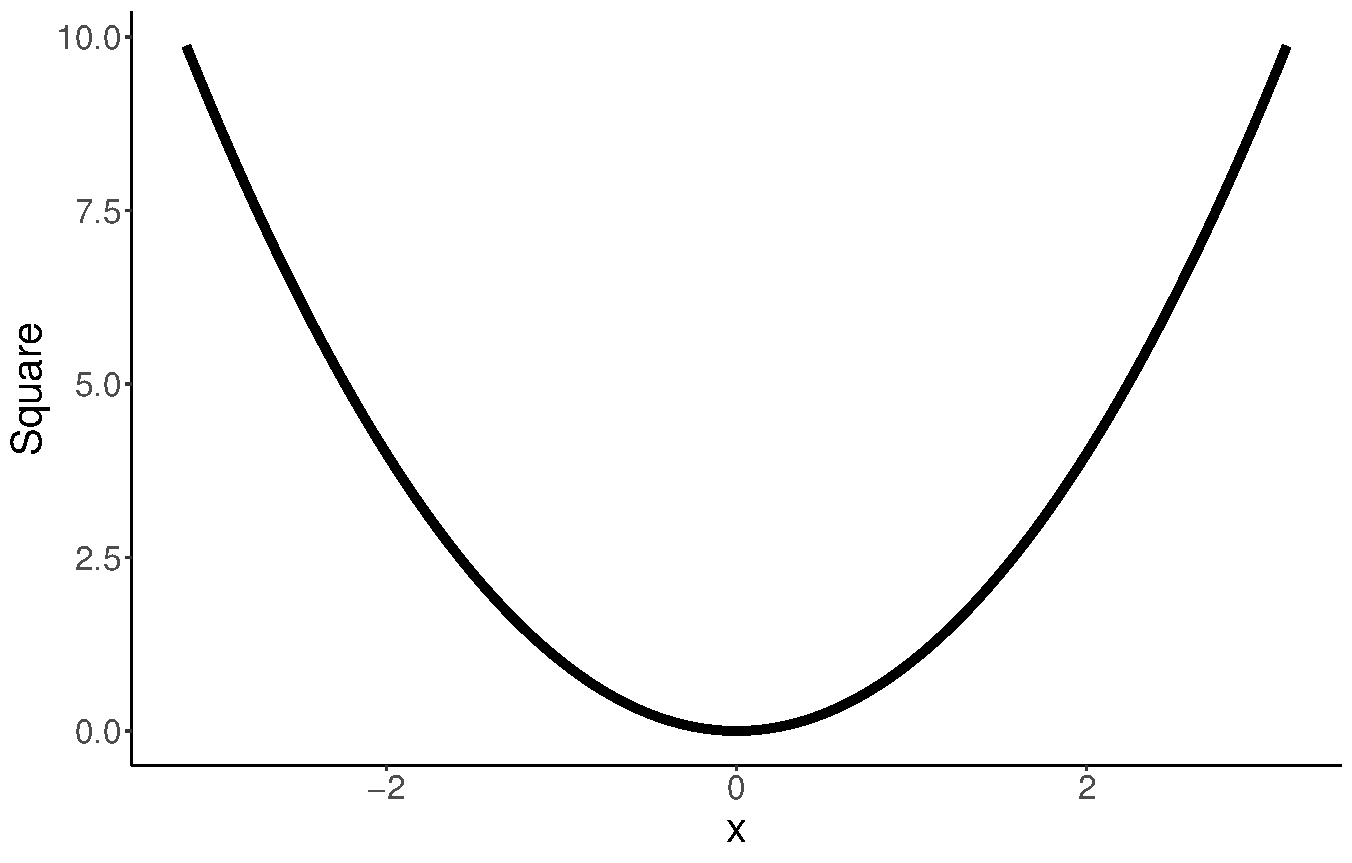
\includegraphics[width=.48\linewidth]{F:/assignment/Figures/square.pdf}
\caption{Square}
\end{figure}
\begin{lstlisting}
# power function

f.power <- function(x,a){
x^a
}
ggplot(data = data.frame(x = seq(-pi,pi,length.out = 500)),aes(x=x)) +
stat_function(fun = f.power, geom = "line", size=2, col="blue",args = (a=1)) +
stat_function(fun = f.power, geom = "line", size=2, col="red",args = (a=2)) +
stat_function(fun = f.power, geom = "line", size=2, col="green",args = (a=3)) +
theme_classic() + 
theme(text = element_text(size = 20)) +
xlab("x") + ylab("Power")
ggsave(file = "F:/assignment/Figures/power.pdf")
\end{lstlisting}
\begin{figure}[hbt]
\centering
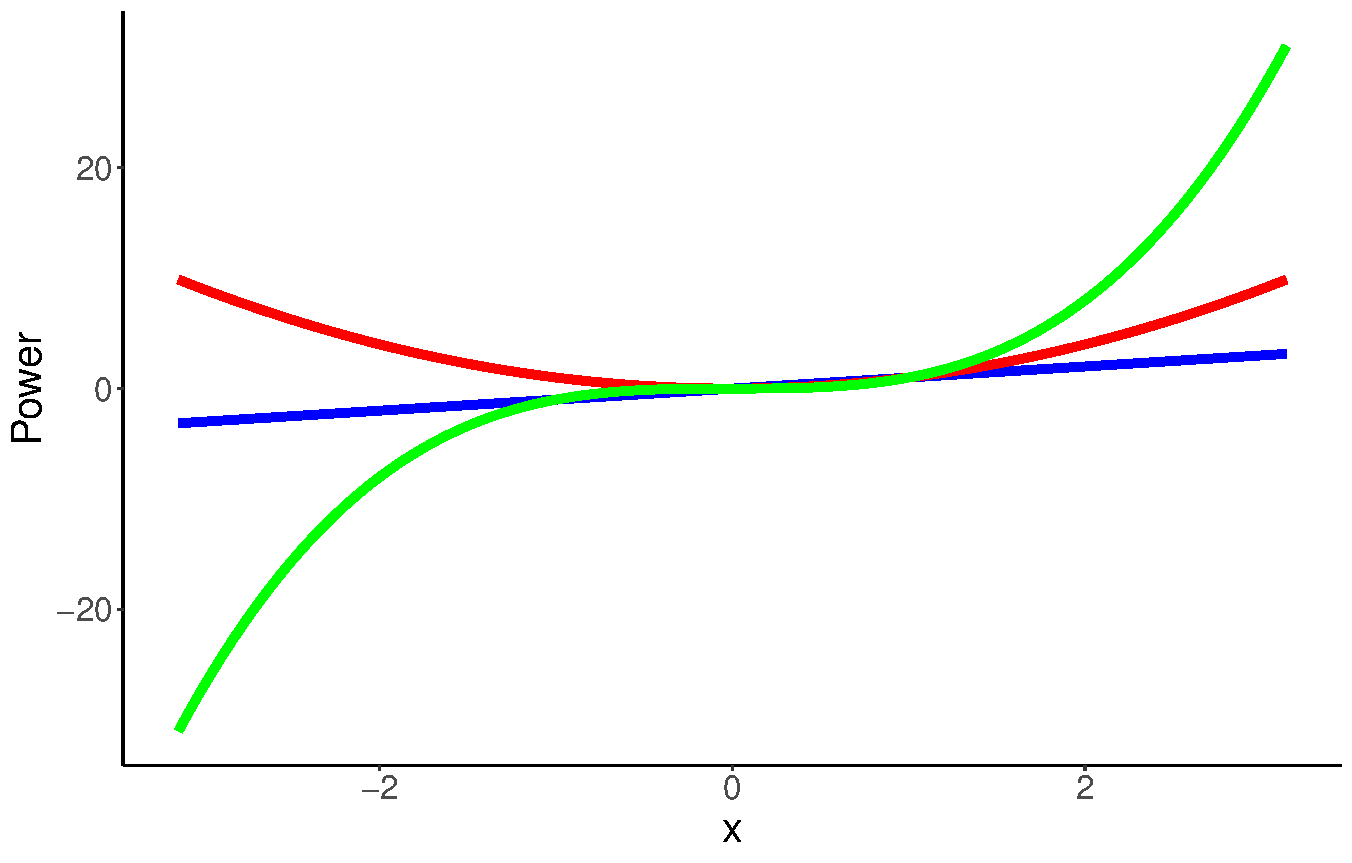
\includegraphics[width=.48\linewidth]{F:/assignment/Figures/power.pdf}
\caption{Power}
\end{figure}
\begin{lstlisting}
# sin(1/x)*x function

f.sinx <- function(x){
x*sin(1/x)
}
ggplot(data = data.frame(x = seq(-pi,pi,length.out = 500)),aes(x=x)) +
stat_function(fun = f.sinx, geom = "line", size=2, col="black") +
theme_classic() + 
theme(text = element_text(size = 20)) +
xlab("x") + ylab("sinx")
ggsave(file = "F:/assignment/Figures/sinx.pdf")
\end{lstlisting}
\begin{figure}[hbt]
\centering
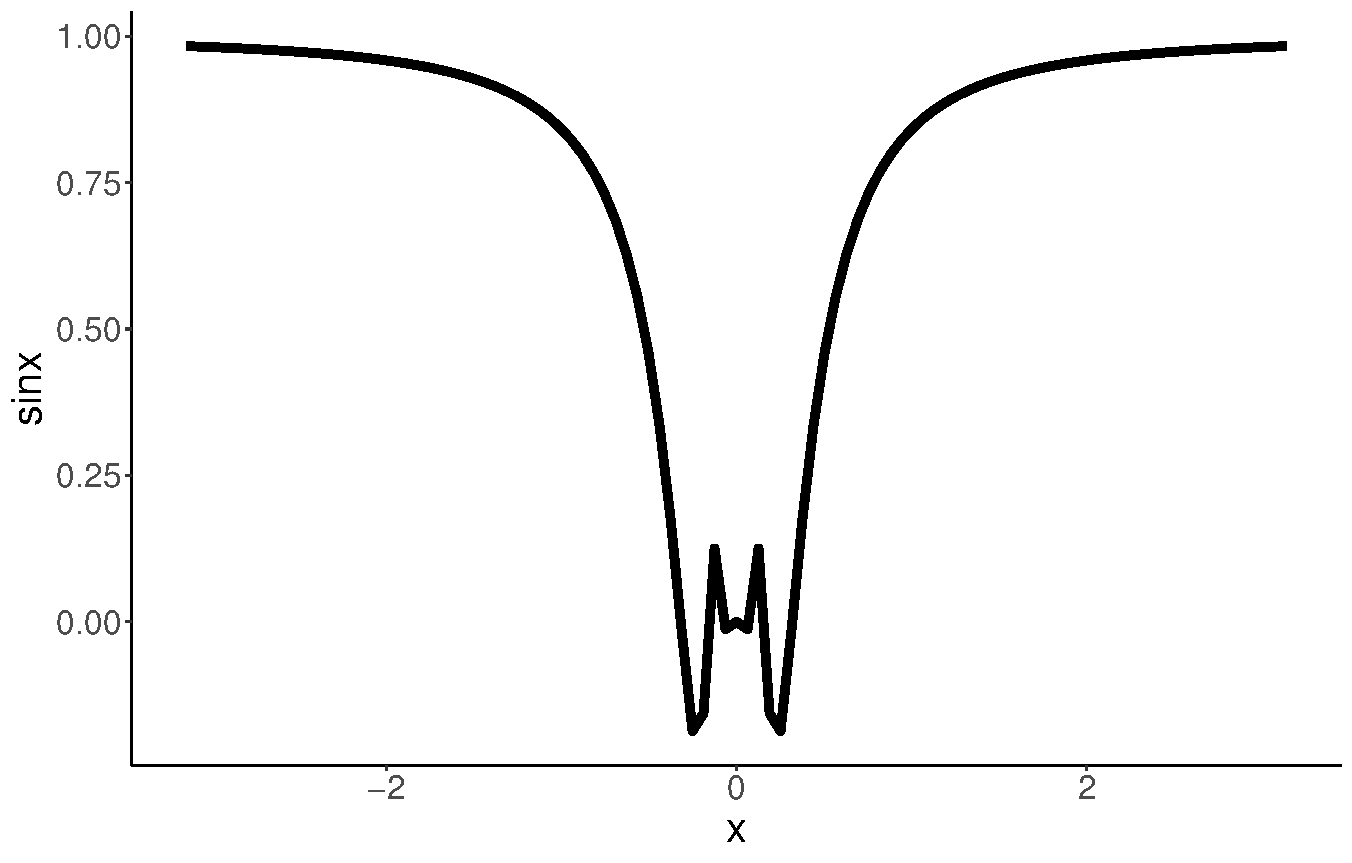
\includegraphics[width=.48\linewidth]{F:/assignment/Figures/sinx.pdf}
\caption{Sinx}
\end{figure}
\textbf{$\mathcal K$-distributed} \\
Implement $\mathcal K$-distributed using R language \\
\begin{lstlisting}
# Intensity K distributions

f.K <- function(x,p_alpha,p_lambda,p_L){
(2*p_lambda*p_L/(gamma(p_alpha)*gamma(p_L)))*((p_lambda*p_L*x)^((p_alpha+p_L)/2-1))*besselK(2*sqrt(p_lambda*p_L*x),p_alpha-p_L)
}
ggplot(data=data.frame(x=seq(0.01, 7, length.out = 500)), aes(x=x)) +
stat_function(fun=dexp, geom = "line", size=2, col="green", args = (mean=1)) +
stat_function(fun=f.K, geom = "line", size=2, col="red", args = list(p_alpha=1, p_lambda=1, p_L=1)) +
stat_function(fun=f.K, geom = "line", size=2, col="blue", args = list(p_alpha=3, p_lambda=3, p_L=1)) +
stat_function(fun=f.K, geom = "line", size=2, col="black", args = list(p_alpha=8, p_lambda=8, p_L=1)) +
theme_classic() +
theme(text = element_text(size=20)) +
xlab("x") + ylab("Intensity K and Exponential Densities")
ggsave(file = "F:/assignment/Figures/KIDensities.pdf")

ggplot(data=data.frame(x=seq(0.01, 7, length.out = 500)), aes(x=x)) +
stat_function(fun=dexp, geom = "line", size=2, col="green", args = (mean=1)) +
stat_function(fun=f.K, geom = "line", size=2, col="red", args = list(p_alpha=1, p_lambda=1, p_L=1)) +
stat_function(fun=f.K, geom = "line", size=2, col="blue", args = list(p_alpha=3, p_lambda=3, p_L=1)) +
stat_function(fun=f.K, geom = "line", size=2, col="black", args = list(p_alpha=8, p_lambda=8, p_L=1)) +
theme_classic() +
theme(text = element_text(size=20)) +
coord_trans(y="log10") +
xlab("x") + ylab("Intensity K and Exponential Densities")
ggsave(file="F:/assignment/Figures/KIDensitiesSemilog.pdf")  

ggplot(data=data.frame(x=seq(0.01, 7, length.out = 500)), aes(x=x)) +
stat_function(fun=f.K, geom = "line", size=2, col="red", args = list(p_alpha=2, p_lambda=2, p_L=1)) +
stat_function(fun=f.K, geom = "line", size=2, col="blue", args = list(p_alpha=2, p_lambda=2, p_L=3)) +
stat_function(fun=f.K, geom = "line", size=2, col="black", args = list(p_alpha=2, p_lambda=2, p_L=8)) +
theme_classic() +
theme(text = element_text(size=20)) +
xlab("x") + ylab("Intensity K densities with varying Looks ")
ggsave(file="F:/assignment/Figures/KIDensitiesLooks.pdf")  

ggplot(data=data.frame(x=seq(0.01, 7, length.out = 500)), aes(x=x)) +
stat_function(fun=f.K, geom = "line", size=2, col="red", args = list(p_alpha=2, p_lambda=2, p_L=1)) +
stat_function(fun=f.K, geom = "line", size=2, col="blue", args = list(p_alpha=2, p_lambda=2, p_L=3)) +
stat_function(fun=f.K, geom = "line", size=2, col="black", args = list(p_alpha=2, p_lambda=2, p_L=8)) +
theme_classic() +
theme(text = element_text(size=20)) +
coord_trans(y="log10") +
xlab("x") + ylab("Intensity K Densities with varying Looks")
ggsave(file="F:/assignment/Figures/KIDensitiesSemilogLooks.pdf")  
\end{lstlisting}
\begin{figure}[hbt]
\centering
\subfloat[Densities]{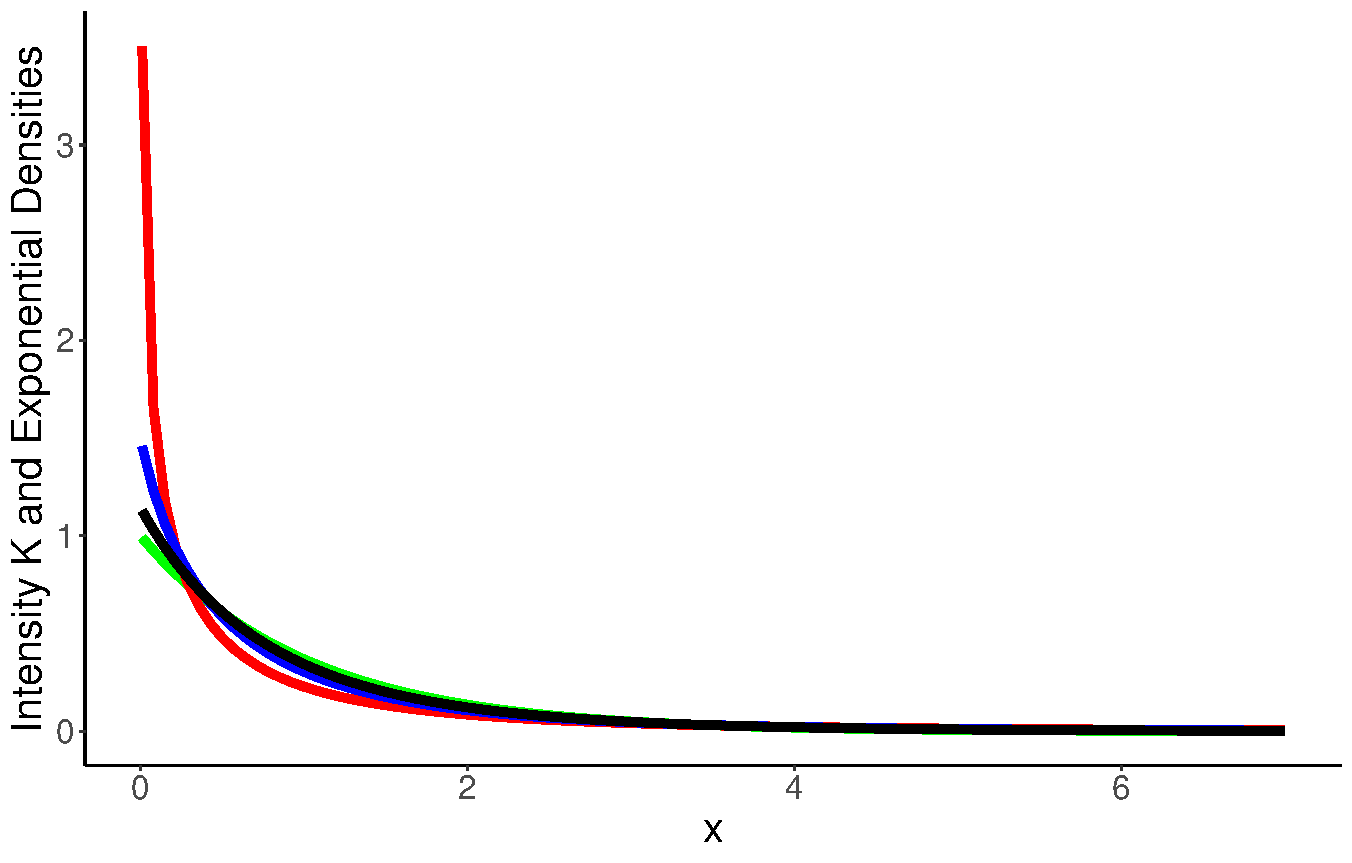
\includegraphics[width=.48\linewidth]{F:/assignment/Figures/KIDensities.pdf}}
\subfloat[Densities in semilog scale]{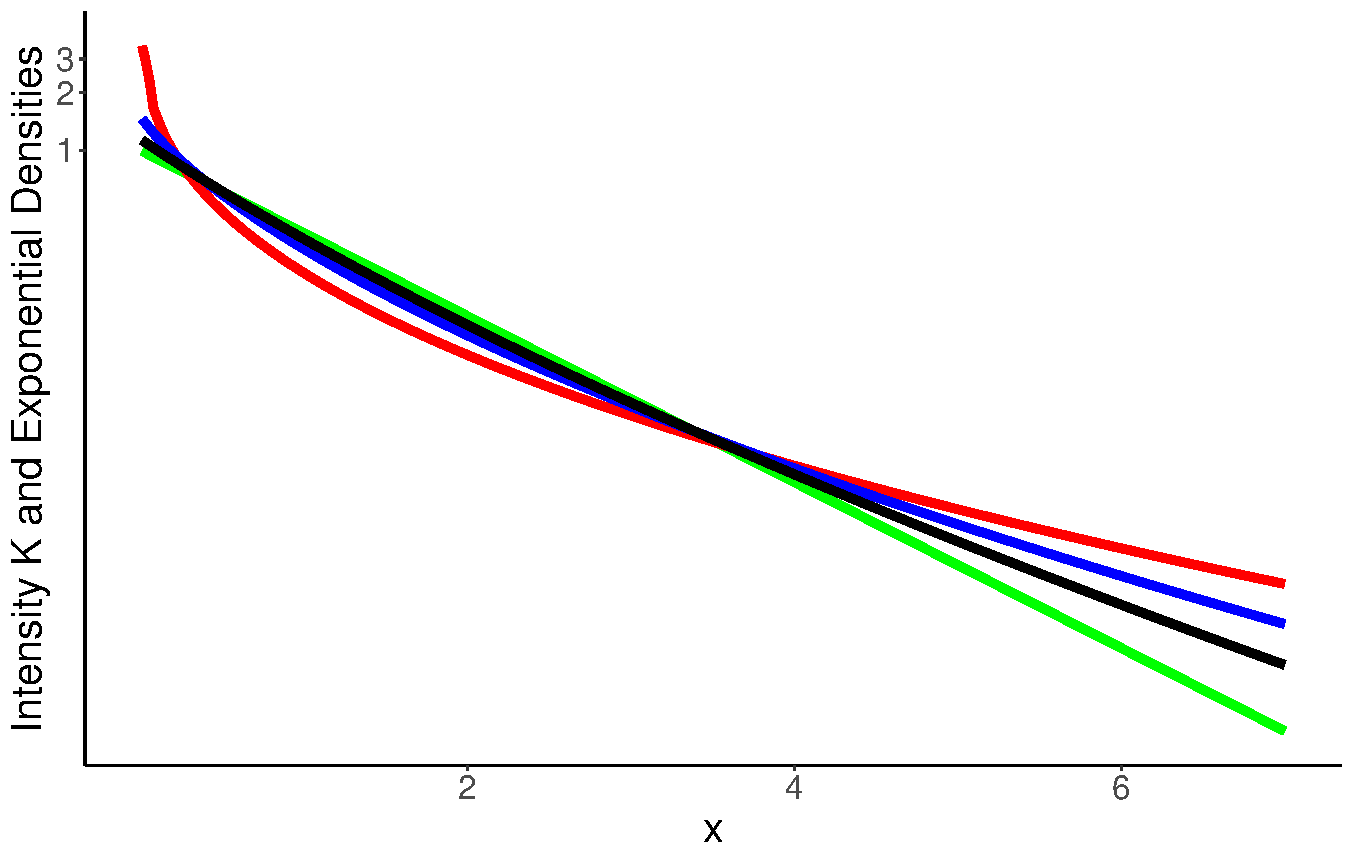
\includegraphics[width=.48\linewidth]{F:/assignment/Figures/KIDensitiesSemilog.pdf}}
\caption[Densities in linear and semilogarithmic scale of the $\text{E}(1)$ (green) and $\mathcal K$ distributions]{Densities in linear and semilogarithmic scale of the $\text{E}(1)$ (green) and $\mathcal K$ distributions with unitary mean ($\alpha\in\{1,3,8\}$ in red, blue, and black, resp.}

	\centering
	\subfloat[Densities]{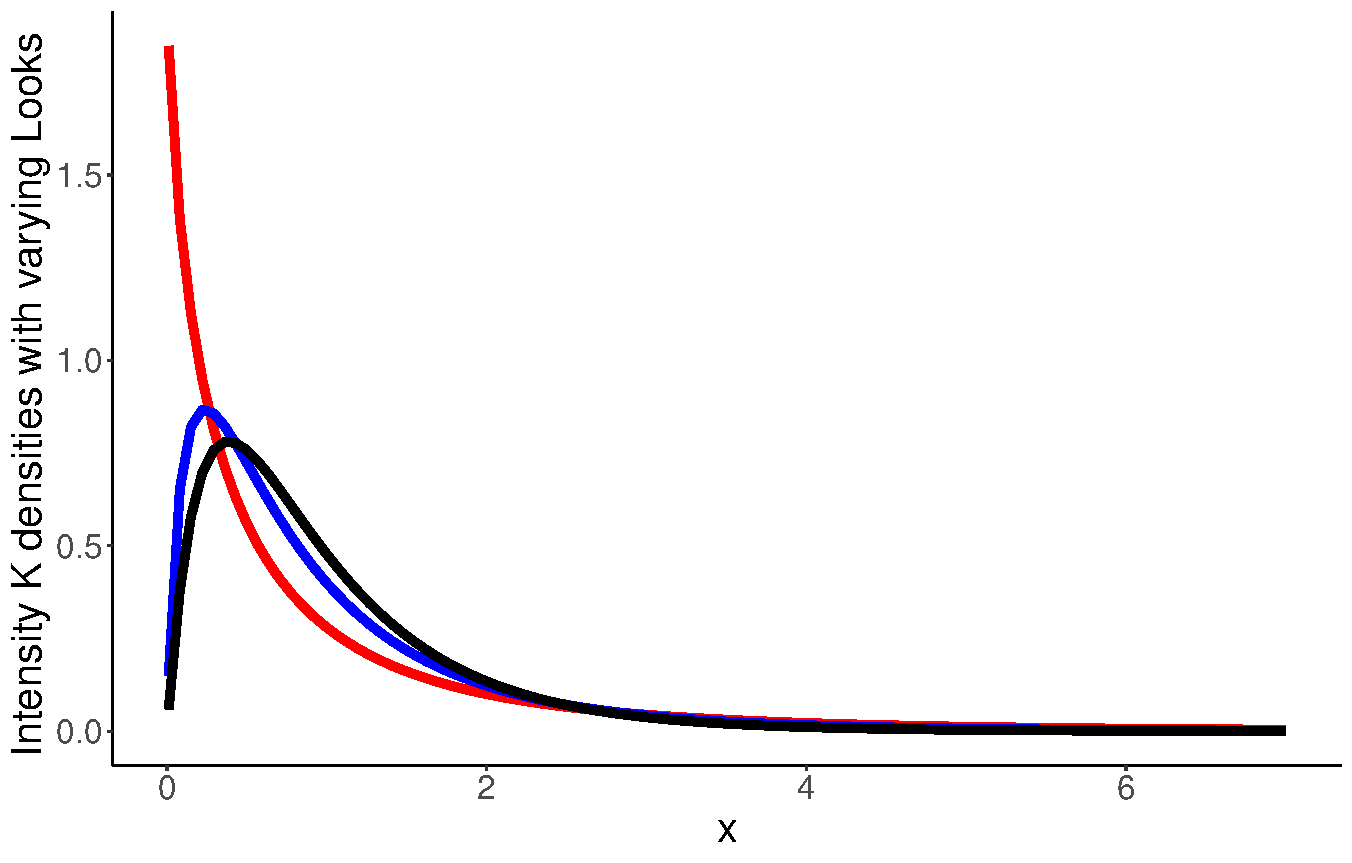
\includegraphics[width=.48\linewidth]{F:/assignment/Figures/KIDensitiesLooks.pdf}}
	\subfloat[Densities in semilog scale]{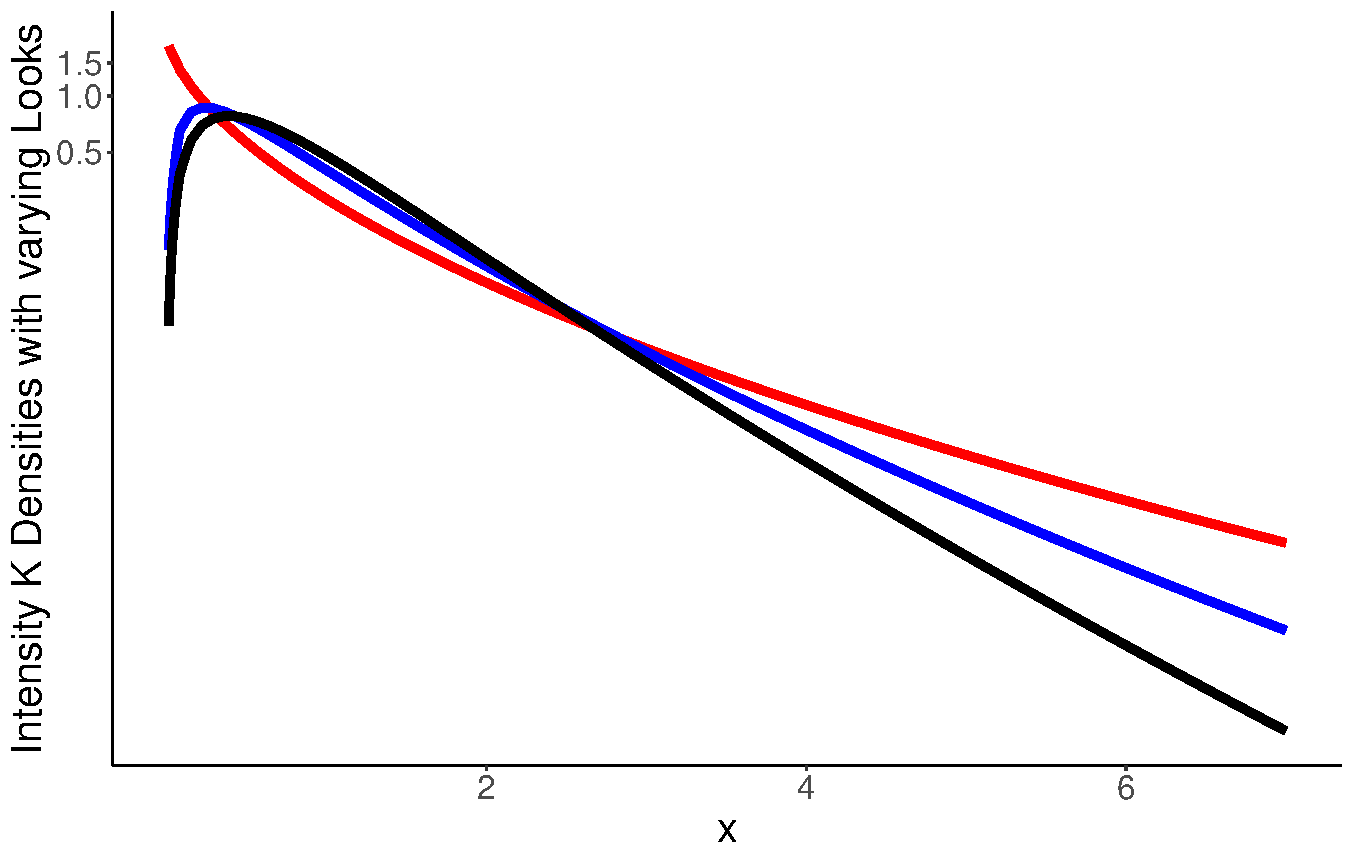
\includegraphics[width=.48\linewidth]{F:/assignment/Figures/KIDensitiesSemilogLooks.pdf}}
	\caption[Densities in linear and semilogarithmic scale $\mathcal K(2,2,L)$ distributions with unitary mean and $L\in\{1,3,8\}$]{Densities in linear and semilogarithmic scale $\mathcal K(2,2,L)$ distributions with unitary mean and $L\in\{1,3,8\}$ in red, blue, and black, resp.}
\end{figure}
\textbf{$\mathcal G^0$-distributed} \\
Implement $\mathcal G^0$ using R language \\
\begin{lstlisting}
# Intensity GI0 distributions

f.GI0 <- function(x,p_alpha,p_gamma,p_L){
((p_L^p_L*gamma(p_L-p_alpha))/(p_gamma^p_alpha*gamma(p_L)*gamma(-p_alpha)))*(x^(p_L-1)/(p_gamma+p_L*x)^(p_L-p_alpha))
}

ggplot(data=data.frame(x=seq(0.01, 10, length.out = 500)), aes(x=x)) +
stat_function(fun=dexp, geom = "line", size=2, col="green", args = (mean=1)) +
stat_function(fun=f.GI0, geom = "line", size=2, col="red", args = list(p_alpha=-1.5, p_gamma=.5, p_L=1)) +
stat_function(fun=f.GI0, geom = "line", size=2, col="blue", args = list(p_alpha=-3, p_gamma=2, p_L=1)) +
stat_function(fun=f.GI0, geom = "line", size=2, col="black", args = list(p_alpha=-8, p_gamma=7, p_L=1)) +
theme_classic() +
theme(text = element_text(size=20)) +
xlab("x") + ylab("Intensity G0 and Exponential Densities")
ggsave(file="F:/assignment/Figures/GI0Densities.pdf")  

ggplot(data=data.frame(x=seq(0.01, 10, length.out = 500)), aes(x=x)) +
stat_function(fun=dexp, geom = "line", size=2, col="green", args = (mean=1)) +
stat_function(fun=f.GI0, geom = "line", size=2, col="red", args = list(p_alpha=-1.5, p_gamma=.5, p_L=1)) +
stat_function(fun=f.GI0, geom = "line", size=2, col="blue", args = list(p_alpha=-3, p_gamma=2, p_L=1)) +
stat_function(fun=f.GI0, geom = "line", size=2, col="black", args = list(p_alpha=-8, p_gamma=7, p_L=1)) +
theme_classic() +
theme(text = element_text(size=20)) +
coord_trans(y="log10") +
xlab("x") + ylab("Intensity G0 and Exponential Densities")
ggsave(file="F:/assignment/Figures/GI0DensitiesSemilog.pdf")  

ggplot(data=data.frame(x=seq(0.01, 10, length.out = 500)), aes(x=x)) +
stat_function(fun=f.GI0, geom = "line", size=2, col="red", args = list(p_alpha=-5, p_gamma=4, p_L=1)) +
stat_function(fun=f.GI0, geom = "line", size=2, col="blue", args = list(p_alpha=-5, p_gamma=4, p_L=3)) +
stat_function(fun=f.GI0, geom = "line", size=2, col="black", args = list(p_alpha=-5, p_gamma=4, p_L=8)) +
theme_classic() +
theme(text = element_text(size=20)) +
xlab("x") + ylab("Intensity G0 densities with varying Looks ")
ggsave(file="F:/assignment/Figures/GI0DensitiesLooks.pdf")  

ggplot(data=data.frame(x=seq(0.01, 10, length.out = 500)), aes(x=x)) +
stat_function(fun=f.GI0, geom = "line", size=2, col="red", args = list(p_alpha=-5, p_gamma=4, p_L=1)) +
stat_function(fun=f.GI0, geom = "line", size=2, col="blue", args = list(p_alpha=-5, p_gamma=4, p_L=3)) +
stat_function(fun=f.GI0, geom = "line", size=2, col="black", args = list(p_alpha=-5, p_gamma=4, p_L=8)) +
theme_classic() +
theme(text = element_text(size=20)) +
coord_trans(y="log10") +
xlab("x") + ylab("Intensity G0 Densities with varying Looks") 
\end{lstlisting}
\begin{figure}[hbt]
\centering
\subfloat[Densities]{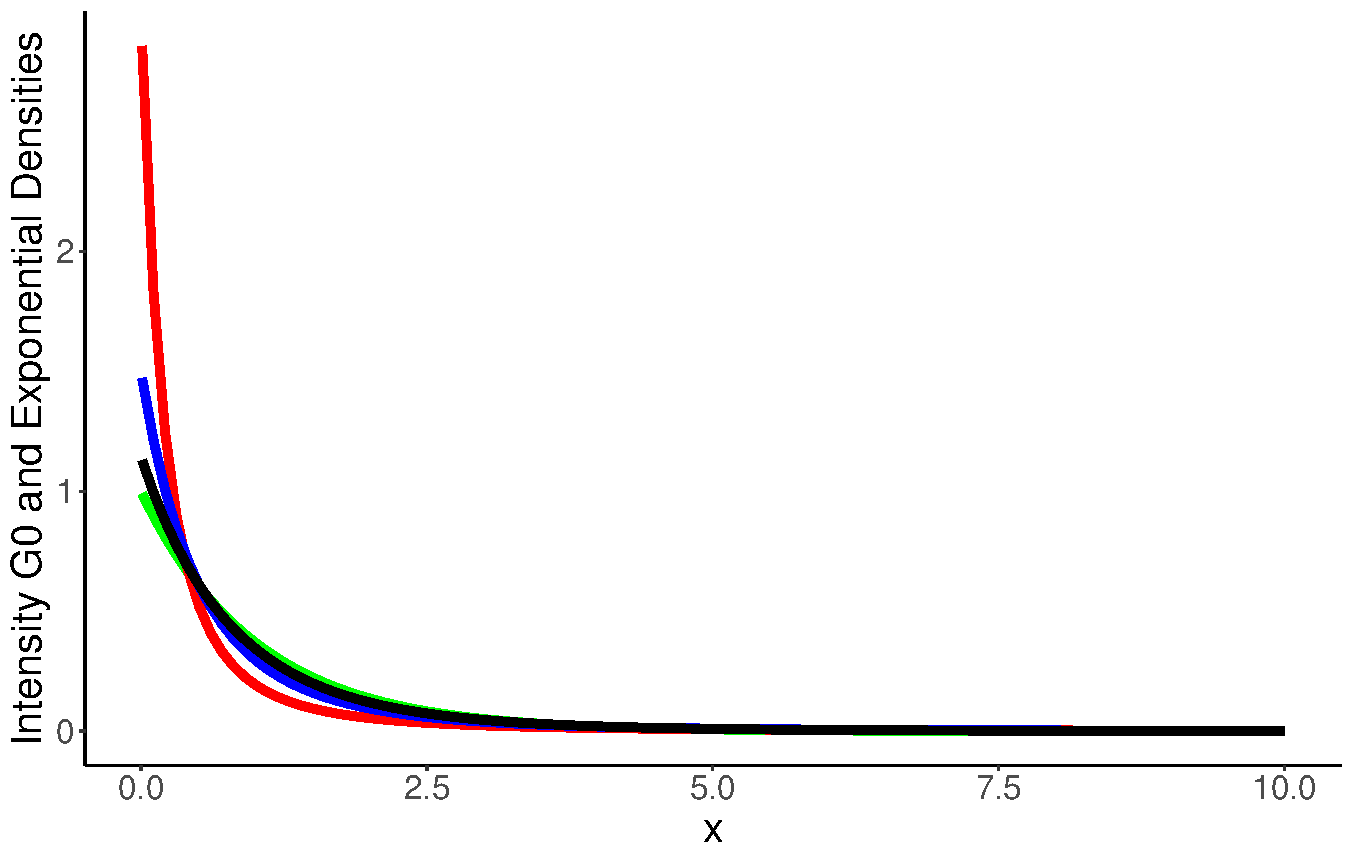
\includegraphics[width=.48\linewidth]{F:/assignment/Figures/GI0Densities.pdf}}
\subfloat[Densities in semilog scale]{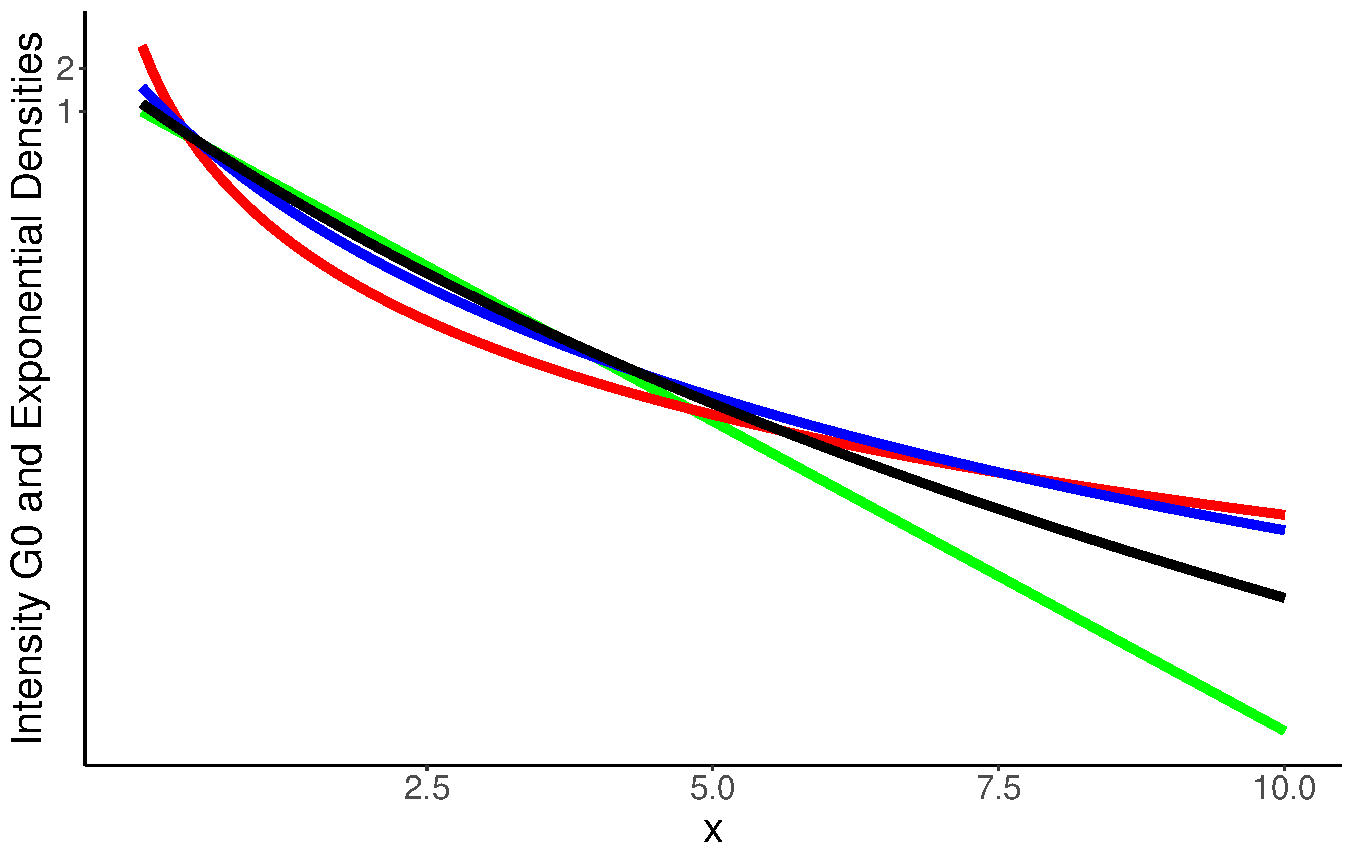
\includegraphics[width=.48\linewidth]{F:/assignment/Figures/GI0DensitiesSemilog.pdf}}
\caption[Densities in linear and semi-logarithmic scale of the $\text{E}(1)$ (green) and $\mathcal G^0$ distributions with unitary mean]{Densities in linear and semi-logarithmic scale of the $\text{E}(1)$ (green) and $\mathcal G^0$ distributions with unitary mean and $\alpha\in\{-1.5,-3,-8\}$ in red, blue, and black, resp.}
\end{figure}
\begin{figure}[hbt]
\centering
\subfloat[Densities]{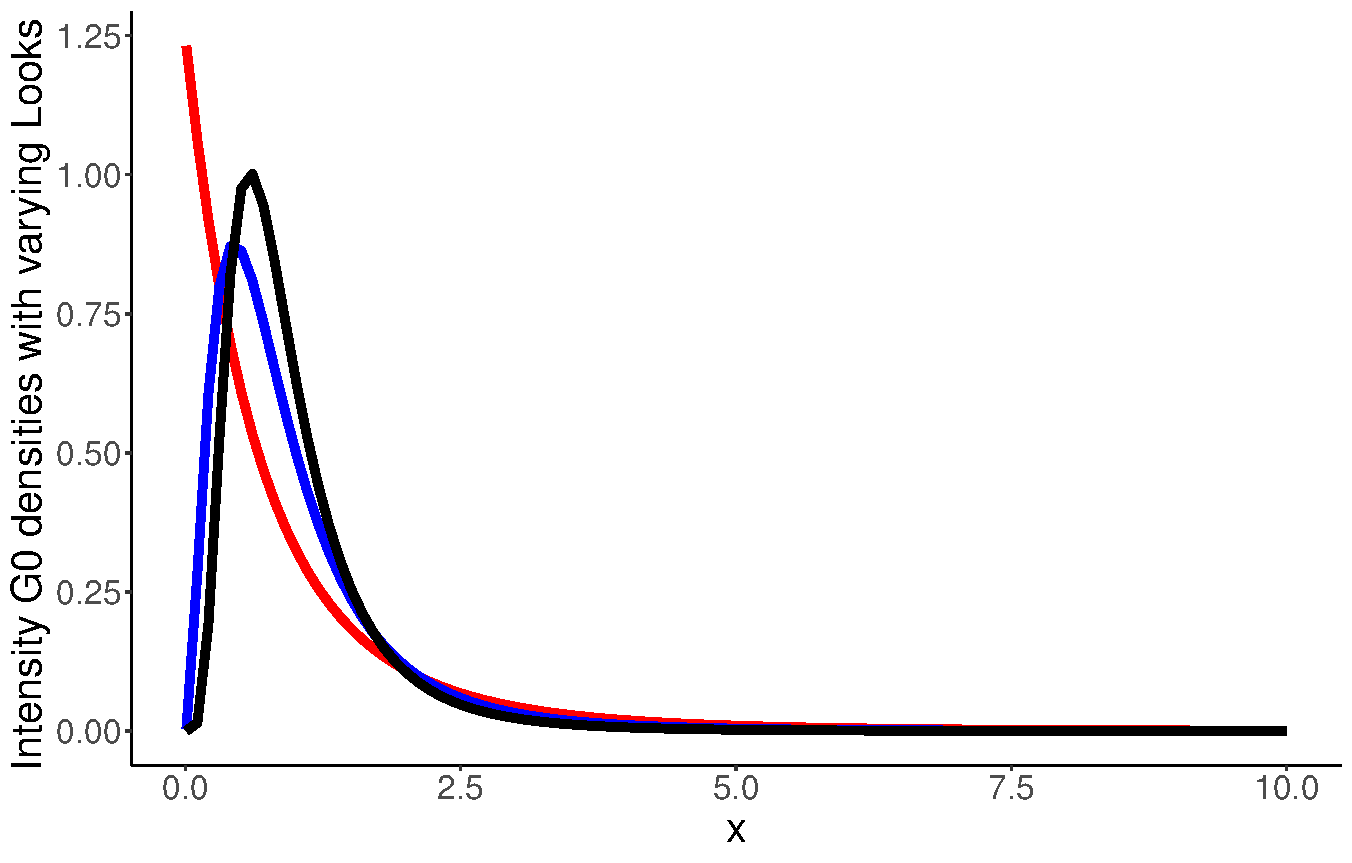
\includegraphics[width=.48\linewidth]{F:/assignment/Figures/GI0DensitiesLooks.pdf}}
\subfloat[Densities in semilog scale]{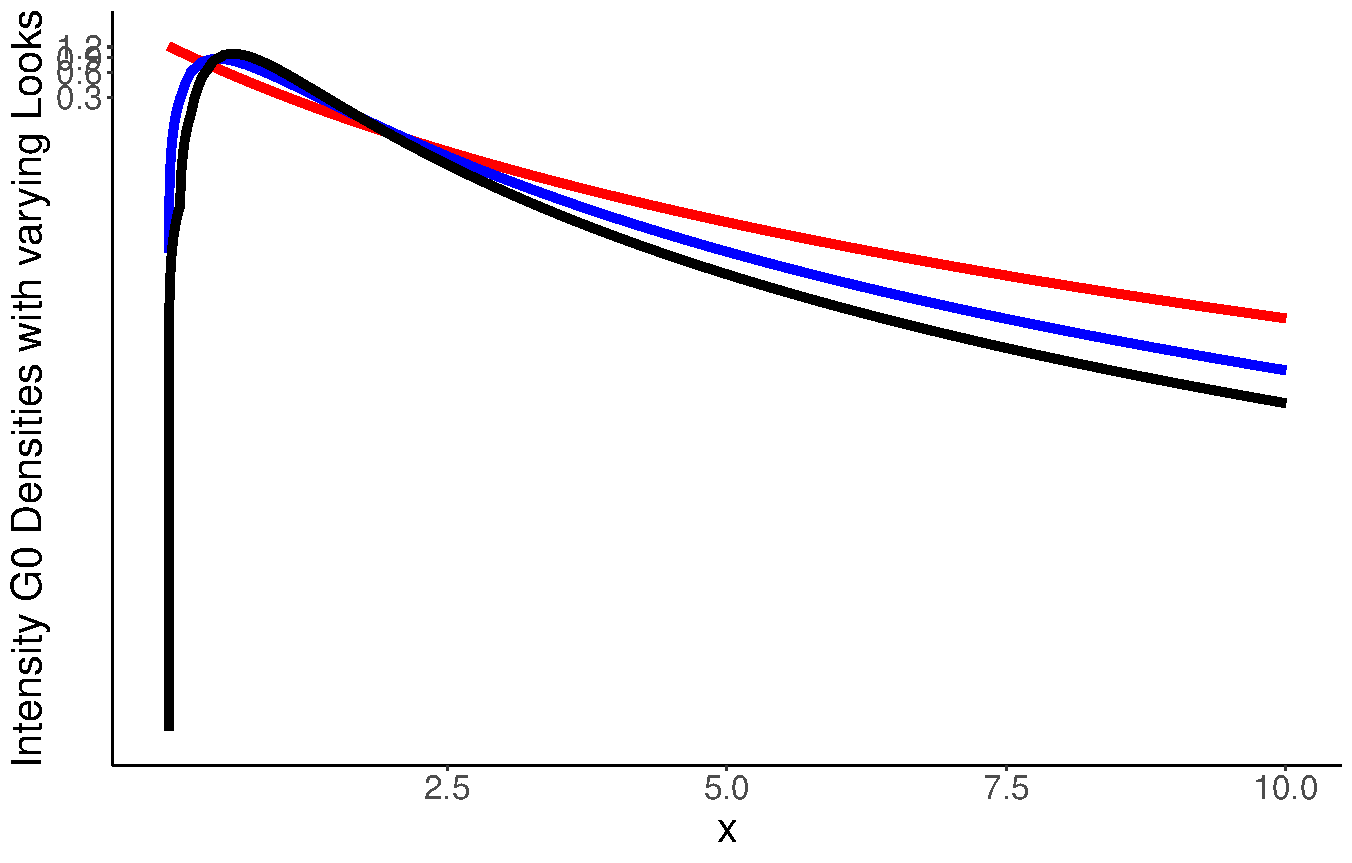
\includegraphics[width=.48\linewidth]{F:/assignment/Figures/GI0DensitiesSemilogLooks.pdf}}
\caption[Densities in linear and semilogarithmic scale $\mathcal G^0(-5,4,L)$ distributions with unitary mean and $L\in\{1,3,8\}$]{Densities in linear and semilogarithmic scale $\mathcal G^0(-5,4,L)$ distributions with unitary mean and $L\in\{1,3,8\}$ in red, blue, and black, resp.}
\end{figure}


% Assignment 4
\section*{Assignment \#4}
\addcontentsline{toc}{section}{Assignment \#4}
\subsection*{Task}
\addcontentsline{toc}{subsection}{Task}
Including today's activities
\subsection*{Activities}
\addcontentsline{toc}{subsection}{Activities}
Solving the maximum likelihood function estimate. \\
\textbf{Step:} \\
\begin{enumerate}
	\item $D(\theta)$
	\item $f_X(\underline{X};\theta)$
	\item $L(\theta;\underline{X})$
	\item $argmax L(\theta;\underline{X})$
\end{enumerate}

% Assignment 5
\section*{Assignment \#5}
\addcontentsline{toc}{section}{Assignment \#5}
\subsection*{Task}
\addcontentsline{toc}{subsection}{Task}
Including today's activities
\subsection*{Activities}
\addcontentsline{toc}{subsection}{Activities}
\textbf{Parameter Estimation} \\
Build estimators to analysis the data from an urban \\
\begin{lstlisting}
# estimator
GI0.Estimator.m1m2 <- function(z,L){
m1 <- mean(z)
m2 <- mean(z^2)
m212 <- m2/m1^2

a <- -2 - (L+1) / (L * m212)
g <- m1 * (2 + (L+1) / (L *m212))

return(list("alpha"=a,"gamma"=g))
}


# LogLikelihoodLknown
LogLikelihoodLknown <- function(params){
p_alpha <- -abs(params[1])
p_gamma <- abs(params[2])
p_L <- abs(params[3])

n <- length(z)

return(
n*(lgamma(p_L-p_alpha) - p_alpha*log(p_gamma) - lgamma(-p_alpha)) + (p_alpha-p_L)*sum(log(p_gamma + z*p_L))
)
}

Intensity_restricted <- subset(vUrbanHV$UHV, subset = vUrbanHV$UHV <= 100000)
binwidth_restricted <- 2*IQR(Intensity_restricted)*length(Intensity_restricted)^(-1/3)
vUrbanHV <- data.frame(UHV=as.vector(UrbanHV[90:200,50:100]))
meanUHV <- mean(vUrbanHV$UHV)
secondUHV <- mean(vUrbanHV$UHV^2)
a <- 2 * (1-CoeffVariation2) / (CoeffVariation2-2)
g <- meanUHV * (-a-1)
z <- vUrbanHV$UHV

estim.Urban <- GI0.Estimator.m1m2(UrbanHV,1)
estim.UrbanML <- maxNR(LogLikelihoodLknown,
start = c(estim.Urban$alpha,estim.Urban$gamma,1),
activePar = c(TRUE,TRUE,FALSE))$estimate[1:2]

ggplot(data=vUrbanHV, aes(x=UHV)) + 
geom_histogram(aes(y=..density..), 
binwidth = binwidth_restricted) + 
xlim(0,200000) +
stat_function(fun=dexp, args=list(rate=1/meanUHV), 
col="red", lwd=2, alpha=.7) +
stat_function(fun=f.GI0, args = list(p_alpha=estim.Urban$alpha, p_gamma=estim.Urban$gamma, p_L=1),
col="blue", lwd=2, alpha=.7) +
stat_function(fun=f.GI0, args = list(p_alpha=estim.UrbanML[1], p_gamma=estim.UrbanML[2], p_L=1),
col="green", lwd=2, alpha=.7) +
xlab("Intensities from the Urban Area") +
ylab("Histogram, and fitted Exponential and G0 Laws") +
ggtitle("Restricted Histogram") +
theme_few()
ggsave(file="F:/assignment/Figures/HistogramRestrictedUrban.pdf")
\end{lstlisting}
\begin{figure}[hbt]
\centering
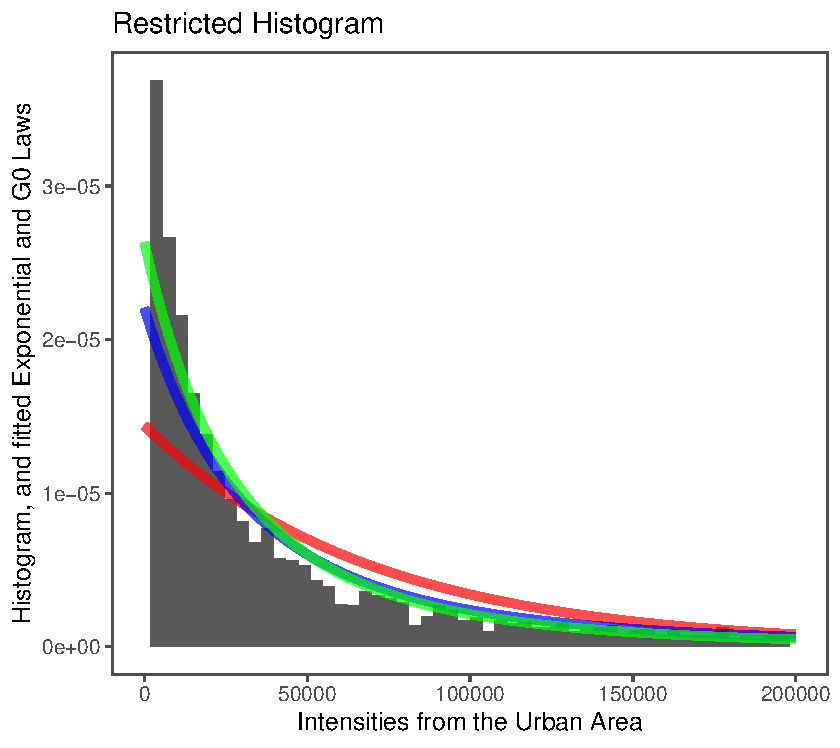
\includegraphics[width=\linewidth]{F:/assignment/Figures/HistogramRestrictedUrbanWFitted.pdf}
\caption{Restricted histogram of the urban area data, with fitted exponential (red) and $\mathcal G^0$ densities; the latter is shown with the parameters estimated by the moments (blue) and maximum likelihood (green) methods.}
\end{figure}
The better quality of the fit with the $\mathcal G^0$ model is noticeable.
There seems to be evidence that the maximum likelihood estimates provide a better fit than that with the moments estimates.

%	BIBLIOGRAPHY
\pagebreak
\bibliography{citepaper} % Use the bibliography.bib file for the bibliography
\bibliographystyle{unsrt}

\end{document}



